\documentclass{beamer}
\usepackage{amsmath}
\usepackage{tikz}
\usetikzlibrary{bayesnet}

\title{Posterior Predictive Distribution}
\author{Oliver Dürr}
\date{\today}

\begin{document}
 
\frame{\titlepage}

\begin{frame}
\frametitle{Intuition}

\[
p(y|D) = \int p(y|\theta) \cdot p(\theta|D) \, d\theta 
\]

\begin{enumerate}
    \item Sample \( \theta_i \sim p(\theta|D) \) (usual posterior samples)
    \item Sample \( y_j \sim p(y|\theta_i) \)
\end{enumerate}
\end{frame}

\begin{frame}
\frametitle{Intuition PPD}

\[
p(y|D) = \int p(y|\theta) p(\theta|D) \, d\theta \quad \text{Continuous}
\]

\[
p(y|D) = \sum_{i=1}^{N} p(y|\theta_i) p(\theta_i|D) \quad \text{Discrete}
\]


\begin{center}
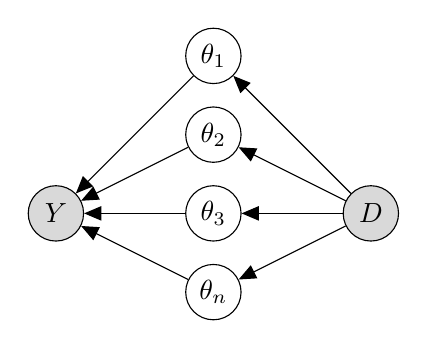
\begin{tikzpicture}
    % Nodes
    \node[obs, fill=gray!30] (y) at (0,0) {$Y$};
    \node[latent] (theta1) at (2,2) {$\theta_1$};
    \node[latent] (theta2) at (2,1) {$\theta_2$};
    \node[latent] (theta3) at (2,0) {$\theta_3$};
    \node[latent] (thetaN) at (2,-1) {$\theta_n$};
    \node[obs, fill=gray!30] (d) at (4,0) {$D$};

    % Edges
    \edge {d} {theta1, theta2, theta3, thetaN};
    \edge {theta1, theta2, theta3, thetaN} {y};
\end{tikzpicture}
\end{center}
\begin{center}
\textit{Getting from a given $D$ to a given $Y$ is nothing more than considering all
the intermediate paths.}
\end{center}
\end{frame}





\begin{frame}
\frametitle{Posterior Predictive (Formal Derivation)}
\begin{tiny}
We are trying to derive the posterior predictive distribution \(P(Y | D)\) for a model with parameters \(\theta\), data \(D\), and a prediction \(Y\). We need the following definitions: \\

\textbf{Definition 1: Conditional Distribution} \\

\[
P(\textcolor{blue}{Y_1}, \textcolor{blue}{Y_2}, \textcolor{blue}{Y_3} | \textcolor{red}{X_1}, \textcolor{red}{X_2}, \textcolor{red}{X_3}) = \frac{P(\textcolor{blue}{Y_1}, \textcolor{blue}{Y_2}, \textcolor{blue}{Y_3}, \textcolor{red}{X_1}, \textcolor{red}{X_2}, \textcolor{red}{X_3})}{P(\textcolor{red}{X_1}, \textcolor{red}{X_2}, \textcolor{red}{X_3})}
\]

\textbf{Definition 2: Marginal Distribution} \\

\[
P(Y_1, Y_2) = \int P(Y_1, Y_2, \textcolor{blue}{Y_3}) \, \textcolor{blue}{dY_3}
\]

\textbf{Derivation of Posterior Predictive Distribution \(P(Y | D)\)} \\
\[
P(Y | D) = \frac{P(Y, D)}{P(D)} \quad \text{(by definition)}
\]
\[
\Rightarrow P(Y | D) = \int \frac{P(Y, D, \theta)}{P(D)} \, d\theta \quad \text{(marginalization over } \theta\text{)}
\]
\[
= \int P(Y | D, \theta) \frac{P(D | \theta) P(\theta)}{P(D)} \, d\theta \quad \text{(chain rule: } P(Y, D, \theta) = P(Y | D, \theta) P(D | \theta) P(\theta)\text{)}
\]
\[
= \int P(Y | D, \theta) P(\theta | D) \, d\theta \quad \text{(Bayes' rule for } P(\theta|D)\text{)}
\]
\[
\text{(Assuming all data relevant to } Y \text{ is captured by } \theta\text{, } P(Y | D, \theta) = P(Y | \theta)\text{)}
\]
\[
P(Y | D) = \int P(Y | \theta) P(\theta | D) \, d\theta \quad \text{(posterior predictive distribution)}
\]

\end{tiny}
\end{frame}

\begin{frame}
    \frametitle{Formal Justification of Posterior Predictive Sampling}
    \textbf{Algorithm:}
    The following algorithm is used to estimate the posterior predictive distribution \( p(y|D) \):
    \begin{enumerate}
        \item Obtain \( N \) posterior samples \( \{\theta_i\}_{i=1}^N \) from \( p(\theta|D) \).
        \item For each posterior sample \( \theta_i \):
        \begin{enumerate}
            \item Draw \( M \) samples \( \{y_{ij}\}_{j=1}^M \) from \( p(y|\theta_i) \).
        \end{enumerate}
        \item Aggregate all \( y_{ij} \) samples to estimate \( p(y|D) \).
    \end{enumerate}
    
    \textbf{Theoretical Justification:}
    \begin{itemize}
        \item \( p(y|D) \) is the expectation of \( p(y|\theta) \) with respect to the posterior distribution \( p(\theta|D) \):
        \[
        p(y|D) = \mathbb{E}_{\theta \sim p(\theta|D)}[p(y|\theta)] = \int p(y|\theta) p(\theta|D) \, d\theta
        \]
        \item This integral is approximated by averaging over the posterior samples.
        \item Often $M=1$ is choosen for an unbiased estimate of $p(y|D)$.
    \end{itemize}
\end{frame}
\end{document} 
